% !TEX program = xelatex
\documentclass[aspectratio=169]{ctexbeamer}
\usetheme{Yzl}

\usepackage{tikz,xcolor-material}
\usepackage[fixed]{fontawesome5}
\usetikzlibrary{positioning,shadows,arrows.meta}

\usefonttheme{professionalfonts}
\setsansfont{Open Sans}
\setmainfont{Sarasa UI SC}
\setmonofont{JetBrainsMono-Regular.ttf}[
  Path = C:/Users/11103475/AppData/Local/Microsoft/Windows/Fonts/,
  BoldFont = JetBrainsMono-Bold.ttf,
  ItalicFont = JetBrainsMono-Italic.ttf,
  BoldItalicFont = JetBrainsMono-Bold-Italic.ttf]
\setmathfont{LibertinusMath-Regular.otf}
\setCJKmainfont{Sarasa UI SC}
\setCJKmonofont{Sarasa Mono SC}

\usetikzlibrary{svg.path}
\definecolor{gG}{RGB}{ 60, 186,  84}
\definecolor{gY}{RGB}{244, 194,  13}
\definecolor{gB}{RGB}{ 72, 133, 237}
\definecolor{gR}{RGB}{219,  50,  54}

\newlength\htG
\protected\def\google{\settoheight{\htG}{G}%
  \begin{tikzpicture}[yscale=-1,scale=(\htG/240pt),baseline=(baseline)]
    \fill[fill=gG] svg {m797.49 249.7h35.975v-240.75h-35.975z};
    \coordinate (baseline) at (current bounding box.south);
    \fill[fill=gB] svg {m246.11 116.18h-116.57v34.591h82.673c-4.0842 48.506-44.44 69.192-82.533 69.192-48.736 0-91.264-38.346-91.264-92.092 0-52.357 40.54-92.679 91.371-92.679 39.217 0 62.326 25 62.326 25l24.22-25.081s-31.087-34.608-87.784-34.608c-72.197-0.001-128.05 60.933-128.05 126.75 0 64.493 52.539 127.38 129.89 127.38 68.031 0 117.83-46.604 117.83-115.52 0-14.539-2.1109-22.942-2.1109-22.942z};
    \fill[fill=gR] svg {m341.6 91.129c-47.832 0-82.111 37.395-82.111 81.008 0 44.258 33.249 82.348 82.673 82.348 44.742 0 81.397-34.197 81.397-81.397 0-54.098-42.638-81.959-81.959-81.959zm0.47563 32.083c23.522 0 45.812 19.017 45.812 49.66 0 29.993-22.195 49.552-45.92 49.552-26.068 0-46.633-20.878-46.633-49.79 0-28.292 20.31-49.422 46.741-49.422z};
    \fill[fill=gY] svg {m520.18 91.129c-47.832 0-82.111 37.395-82.111 81.008 0 44.258 33.249 82.348 82.673 82.348 44.742 0 81.397-34.197 81.397-81.397 0-54.098-42.638-81.959-81.959-81.959zm0.47562 32.083c23.522 0 45.812 19.017 45.812 49.66 0 29.993-22.195 49.552-45.92 49.552-26.068 0-46.633-20.878-46.633-49.79 0-28.292 20.31-49.422 46.741-49.422z};
    \fill[fill=gB] svg {m695.34 91.215c-43.904 0-78.414 38.453-78.414 81.613 0 49.163 40.009 81.765 77.657 81.765 23.279 0 35.657-9.2405 44.796-19.847v16.106c0 28.18-17.11 45.055-42.936 45.055-24.949 0-37.463-18.551-41.812-29.078l-31.391 13.123c11.136 23.547 33.554 48.103 73.463 48.103 43.652 0 76.922-27.495 76.922-85.159v-146.77h-34.245v13.836c-10.53-11.347-24.93-18.745-44.04-18.745zm3.178 32.018c21.525 0 43.628 18.38 43.628 49.768 0 31.904-22.056 49.487-44.104 49.487-23.406 0-45.185-19.005-45.185-49.184 0-31.358 22.619-50.071 45.66-50.071z};
    \fill[fill=gR] svg {m925.89 91.02c-41.414 0-76.187 32.95-76.187 81.57 0 51.447 38.759 81.959 80.165 81.959 34.558 0 55.768-18.906 68.426-35.845l-28.235-18.787c-7.3268 11.371-19.576 22.484-40.018 22.484-22.962 0-33.52-12.574-40.061-24.754l109.52-45.444-5.6859-13.318c-10.58-26.08-35.26-47.86-67.92-47.86zm1.4268 31.413c14.923 0 25.663 7.9342 30.224 17.447l-73.139 30.57c-3.1532-23.667 19.269-48.017 42.915-48.017z};
  \end{tikzpicture}%
}

% just for the testing section
% \newcommand{\testing}[1]{\noindent\leavevmode#1\rlap{G}\google\llap{e} \quad \rlap{Google}\google \qquad \google\llap{Google}\par}

\newlength\htK\newlength\dpl
\protected\def\kotlin{\settoheight{\htK}{K}\settodepth{\dpl}{l}%
\raisebox{-\dpl}{
\includegraphics[height=\htK+\dpl]{fig/Kotlin-logo.png}}}

\definecolor{android}{HTML}{30d780}

% \newfontfamily\opensans{Open Sans}
% \newcommand{\google}{{\bfseries\opensans{\color{GoogleBlue}G}{\color{GoogleRed}o}%
%   {\color{GoogleYellow}o}{\color{GoogleBlue}g}{\color{GoogleGreen}l}{\color{GoogleRed}e}}}


\title{\ttfamily{Kotlin} 入坑指北}
\date{\today}
\author{\bfseries 叶至灵}
% \institute{AI 系统中心}

\begin{document}

\maketitle

\begin{frame}[c]
    \frametitle{目录}
    \bfseries
    \tableofcontents[hideallsubsections]
    \thispagestyle{empty}
\end{frame}

\section{为什么选择 \ttfamily{Kotlin}}%
\begin{frame}[fragile]
    \frametitle{历史}
    \begin{columns}
        \begin{column}{0.5\textwidth}
            \begin{itemize}
                \item \textbf{2011} |JetBrains| 发布,面向 JVM
                \item \textbf{2016} |v1.0| 发布
                \item \textbf{2017} \google{} 宣布在{\color{android}\faAndroid}Android 提供 Kotlin 的最佳支持
                \item \textbf{2019} 已作为{\color{android}\faAndroid}Android 开发的推荐语言
            \end{itemize}
        \end{column}
        \begin{column}{0.5\textwidth}
            \begin{figure}
            \begin{center}
                
\includegraphics[height=1cm]{fig/Kotlin}\\
                \vspace{12pt}
                
\includegraphics[height=2cm]{fig/android}
            \end{center}
            \end{figure}
        \end{column}
    \end{columns}
\end{frame}

\begin{frame}[t,fragile]
    \frametitle{特性}
    \begin{quotebox}
        让开发人员更快乐的一门现代编程语言$^1$。
    \end{quotebox}
    \nonumberfootnote{$^1$出自 Kotlin 语言中文站\link{https://www.kotlincn.net/}}
    \vspace{12pt}
    \begin{columns}[t]
        \begin{column}{0.4\textwidth}
            \begin{block}{\faCut 简洁}
                数据类\\
                函数式编程\\
                单例
            \end{block}
        \end{column}
        \begin{column}{0.4\textwidth}
            \begin{block}{\faHardHat 安全}
                空安全\\
                自动类型转换
            \end{block}
        \end{column}
    \end{columns}
    \begin{columns}[t]
        \begin{column}{0.4\textwidth}
            \begin{block}{\faPuzzlePiece 互操作性}
                Java\\
                Android
            \end{block}
        \end{column}
        \begin{column}{0.4\textwidth}
            \begin{block}{\faWrench 工具友好}
                Java IDE\\
                命令行\\
                Jupyter
            \end{block}
        \end{column}
    \end{columns}
\end{frame}

\begin{frame}[fragile]
    \frametitle{\texttt{Why Kotlin?}}
    \begin{columns}
        \begin{column}{0.5\textwidth}
            \begin{itemize}
                \item 越来越多应用通过 |Kotlin| 开发
                \item 用更\textcolor{yzlblue}{短}的代码写出更\textcolor{yzlblue}{安全}的应用
                \item 学习现代编程语言的新特性\\类型推断、函数式编程、协程……
            \end{itemize}
        \end{column}
        \begin{column}{0.5\textwidth}
            \begin{figure}
            \begin{center}
                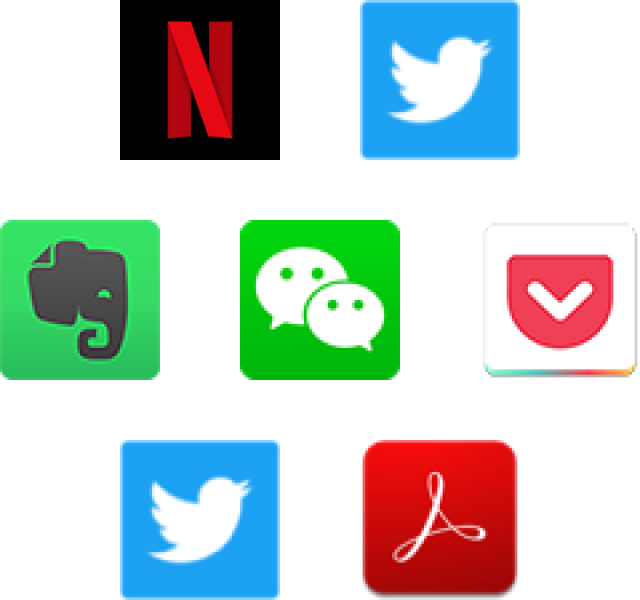
\includegraphics[height=3cm]{fig/apps.png}
            \end{center}
            \end{figure}
        \end{column}
    \end{columns}
\end{frame}

\section{和NPE说再见}

\section{再短一点}

\section{Fun with Android}

\begin{frame}[fragile]
\frametitle{示例}
\begin{kotlincode}[basicstyle=\scriptsize\ttfamily,emph={[1]level}]
/**
 * 按照层级取出编码
 *
 * eg. "000a00".extract(2) -> "000a"
 */
fun String.extact(level: Int) = when (level) {
    0 -> this
    else -> this.substring(0, 2 * level)
}
\end{kotlincode}
\end{frame}

\section{参考}
\begin{frame}[fragile]
\frametitle{参考文献}
\begin{multicols}{2}
\newcommand\BOOK[1]{\textbf{#1}}
\newcommand\TAG[1]{[#1]}
\begin{thebibliography}{99}
  \bibitem{}
    林莲枝.
    \newblock \BOOK{漫谈 \LaTeX{} 排版常见概念误区:别把 \LaTeX{} 当 Word 用!}\TAG{EB/OL}. 2018.
    \newblock PDF:
      \href{http://static.latexstudio.net/wp-content/uploads/2018/03/LianTze-presentation-0320-forReading.pdf}{\faDownload}
  \bibitem{}
    Wikibooks.
    \newblock \BOOK{\LaTeX{}---Wikibooks, The Free Textbook Project} \TAG{EB/OL}.
    \newblock \url{https://en.wikibooks.org/wiki/LaTeX}
  \bibitem{}
    刘庆.
    \newblock \BOOK{孔雀计划:中文字体排印的思路} \TAG{EB/OL}.
    \newblock \url{https://thetype.com/kongque}
\end{thebibliography}
\end{multicols}
\end{frame}

\begin{frame}{关于}
\begin{table}[]
\begin{tabular}{cll}
\faPaintRoller & \textbf{主题}     & Yzl            \\
\faFont        & \textbf{正文字体} & 更纱黑体 + Roboto  \\
\faTextWidth   & \textbf{等宽字体} & \texttt{JetBrains Mono} \\
\end{tabular}
\end{table}
\end{frame}

\begin{frame}[c,fragile]
\frametitle{调色板}
\begin{center}
\colorpalette[primary palette={yzlblue,yzlgreen,yzlgray}, secondary palette={},
primary variation=logoyellow, init text color=white, title text color=logoblack, title font=\bfseries, variation font=\ttfamily]{}
\colorpalette[primary palette={yzlred,yzlorange,yzlpink}, secondary palette={},
primary variation=logoblack, init text color=white, title text color=logoyellow, title font=\bfseries, variation font=\ttfamily]{}
\end{center}
\end{frame}

\begin{frame}[standout]
\begin{center}
\end{center}
\begin{center}
    \begin{tikzpicture}
        \node[anchor=center,inner sep=0,opacity=0.5] at (current page.center) {
\includegraphics[width=4cm]{fig/logo_color.pdf}};
        \node[align=center,logoblack,font={\Huge\ttfamily}] at (current page.center) {Happy \textit{\textbackslash Coding}};
    \end{tikzpicture}
\end{center}
\end{frame}

\end{document}
